\subsection{Fixed Total Cells Do Not Isolate Subject Breadth}
\label{sec:results:patient_cell_scaling}

We begin with the conventional label-agnostic design: outer-test subjects remain
fixed while a constant number of training cells is reallocated from 8 to 32
subjects. Across APT, COMBAT, and OneK1K, 37 of 38
model--resolution--budget comparisons favor greater subject breadth. The
direction appears strikingly consistent across assays and cohorts.

It is not an isolated subject effect. Increasing the number of sampled subjects
also changes which labels are observed, how the fixed cell budget is distributed
among classes, and the resulting class proportions. For example, the mean
number of observed fine classes rises with subject count in all three datasets,
despite fixed total cells. Training-subset intervals are also much less stable
than intervals that condition on the averaged training subsets and bootstrap
only test subjects. The label-agnostic experiment therefore measures a total
allocation effect, not a label-standardized effect. Conditioning on completed
training subsets also omits sensitivity to alternative development samples.

\subsection{Breadth Estimates Depend on the Allocation Policy}
\label{sec:results:class_matched}

The matched comparison freezes the $P=8$ observed class set and exact
per-class quotas, then samples those same quotas from 8 and 32 subjects. Every
joint replicate first selects one completed training-subset seed and then
resamples paired outer-test subjects. This targets the residual effect of
redistributing a fixed class-matched cell budget across more subjects. The
resulting interval describes joint stability, not precision of the seed mean.

\begin{figure}[t]
\centering
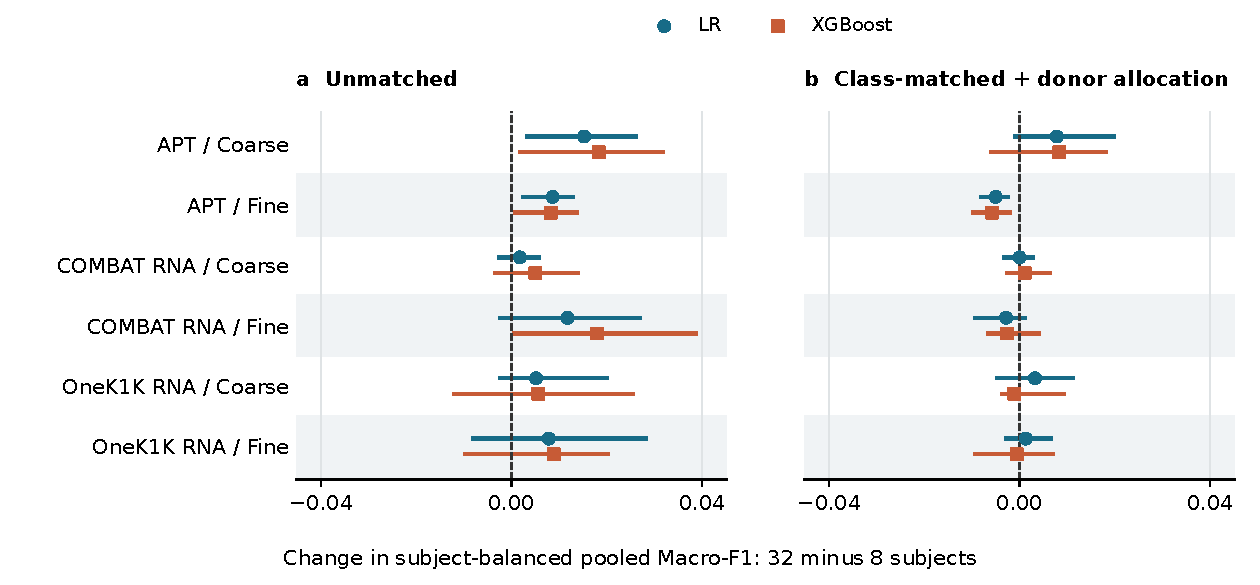
\includegraphics[width=\columnwidth]{figures/scaling_protocol_contrast.pdf}
\caption{The apparent breadth advantage changes under the matched protocol.
Both panels show the change in subject-balanced pooled OOF macro-F1 from 8 to
32 training subjects at $T=6{,}400$, on identical axes. The right panel fixes
class support and exact quotas and additionally uses within-class donor round
robin; this is not a label-only intervention. Points are seed means; bars in
both panels are empirical 2.5th--97.5th seed percentiles, not confidence
intervals of the mean. Unmatched runs and matched LR use 20 seeds; matched
XGBoost uses 10. APT and COMBAT fine point estimates change sign for both models.
Cross-panel changes are descriptive, not paired attenuation tests. The matched
joint stability intervals, which additionally resample held-out subjects, all span zero
(Figure~\ref{fig:class_matched_joint}).}
\label{fig:class_matched_scaling}
\end{figure}

The matched policy yields a different pattern
(Figure~\ref{fig:class_matched_scaling}). At $T=6{,}400$, LR/XGBoost effects
are $+0.0078/+0.0083$ for APT coarse but $-0.0050/-0.0058$ for APT fine.
COMBAT effects are approximately zero for coarse and $-0.0028/-0.0027$ for
fine. OneK1K effects are small and change sign across models. All 12 joint
stability intervals include zero. The APT and COMBAT fine point-estimate
reversals are therefore not specific to a linear classifier, but their signs
are not stable across joint resampling. This is a
joint sampling-protocol contrast: the implementation fixes observed labels,
class counts, and proportions and also uses within-class donor round robin.
The attenuation cannot therefore be assigned solely to label distribution.
An independently controlled synthetic check separates quota matching from donor
allocation (Section~\ref{sec:appendix:sequential_simulation}). The completed
real-cohort separation in Section~\ref{sec:sequential_completed} retains
positive fine effects under exact quotas alone, demonstrating the importance
of distinguishing quota matching from donor allocation. A complementary known-null
validation yields mean effects $+0.0202$, $+0.0119$, and $+0.0004$ for unmatched,
support-matched, and exact-quota sampling against an exactly zero overlap-quota
target. Independent Monte Carlo references under donor shifts remain positive
and are not mechanically removed by matching
(Section~\ref{sec:appendix:known_target}). This checks recovery of a specified
allocation target, not interval coverage or a universal causal effect of subject breadth.

Beyond the common 32-subject grid, class-matched LR
frontiers through 64 COMBAT and 128 OneK1K training donors yield adjacent
mean effects between $-0.00065$ and $+0.00123$, with every joint stability interval
spanning zero. These ranges do not test mean equivalence or a plateau. A post-hoc
$\pm0.01$ sensitivity band contains 11 of 12 adjacent frontier stability intervals,
but only 4 of 12 main $T=6{,}400$ intervals and none of the four APT intervals
(Section~\ref{sec:appendix:equivalence}). These are pointwise interval-containment
diagnostics, not equivalence tests or an optimal-allocation result. Complete unmatched
grids, class-support audits, matched doublings, extended frontiers, and
uncertainty decompositions appear in
Section~\ref{sec:appendix:fair_scaling}--
\ref{sec:appendix:extended_subject_frontier}.
